\section{Desarrollo}
\subsection{Lectura de Giroscopio}
El primer punto que se debe resolver es realizar la lectura de los valores en los ejes X, Y y Z del giroscopio. Para realizar esta sección, se utilizó parte del código que se proporciona por los ejemplos de libopemcm3, esto para funciones no relevantes para los objetivos de este laboratorio, como configurar el reloj del sistema por ejemplo.\\
En la figura \ref{codig1} se muestra el código utilizado para configurar los pines y el SPI5, estos son los elementos necesarios para comunicarse con el giroscopio. Primero se configuran los puertos GPIO, como salidas, así como las frecuencias, luego se configuran los registros SPI5 para habilitarlo a funcionar en modo maestro, dados los parámetros de funcionamiento de la interfaz SPI5 del giroscopio. Es importante mencionar que el orden en el que se llaman estas funciones es el orden que se indica en las diapositivas del curso.

\begin{figure}[H]
    \centering
    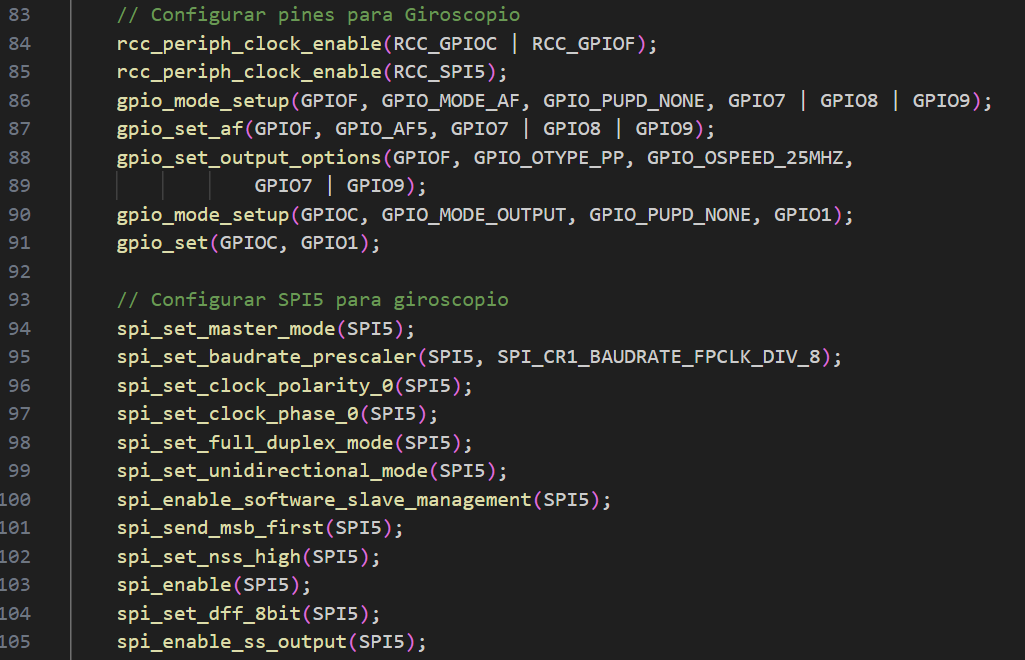
\includegraphics[scale=.5]{Imagenes/codig1.png}
    \caption{Codigo para configurar comunicación con SPI5}
    \label{codig1}
\end{figure}

Luego de realizar estas configuraciones, se pueden configurar los registros del giroscopio y proceder a leer los registros correspondientes a los valores X, Y y Z, tal como se muestra en la figura \ref{codig2}

\begin{figure}[H]
    \centering
    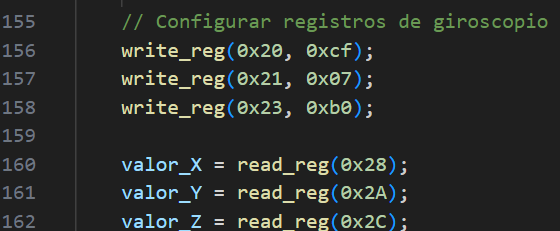
\includegraphics[scale=.5]{Imagenes/codig2.png}
    \caption{Escritura y lectura de registros del giroscopio.}
    \label{codig2}
\end{figure}


Nota importante: Se realizaron múltiples intentos de establecer la comunicación con el giroscopio, desde modificaciones en la configuración de SPI5, simular las comunicaciones SPI5 manualmente, probar ejemplos proporcionados hasta probar codigo proporcionado por compañeros del curso a los cuales sí les funcionaba, sin embargo, no fue posible obtener datos fuera de un constante valor de 0, por ello se llegó a la conclusión de que puede existir algún daño físico en la placa, lo que impide la comunicación con el giroscopio, o que el daño existe en sí en el giroscopio.\\
Para compensar esta carencia, se comentó esta sección del código (en teoría el código sigue siendo funcional y se podría utilizar en una placa en buen estado) y se agregaron unos contadores que simulan el cambio en los valores que proporcionaría el giroscopio. Más adelante en la sección de resultados se mostrará este funcionamiento.

\subsection{LED's, botón y ADC}
Para realizar la configuración de los leds que se usarán para indicar que la tensión de la batería está baja, que la comunicación USART está activada, del botón para habilitar esta comunicación y del convertidor analógico digital, se realizó un proceso de configuración muy similar al que se utilizó para configurar la comunicación con el giroscopio, con la diferencia del cambio de los pines. Así que para evitar extender este reporte, se omite agregar esta sección del código.\\
Fuera de la configuración, en la figura \ref{codig3} se muestra el codigo con la lógica para controlar estas funciones. En las lineas 192-164 se muestra la lógica para encender el led cuando se presiona el botón, esta información se utiliza también para habilitar la comunicación USART. En las lineas 165-167 se muestra el código que se encarga de leer la información sobre la tensión de la batería. En este caso esta información muestra la tensión en mili-volts, para aprovechar la precisión del ADC. Finalmente en las lineas 169-177 se muestra la lógica que se utiliza para encender y apagar el led de color rojo, esta función se activa cuando la tensión es inferior a 7.5V, por lo que se acerca a la tensión de peligro de 7V.

\begin{figure}[H]
    \centering
    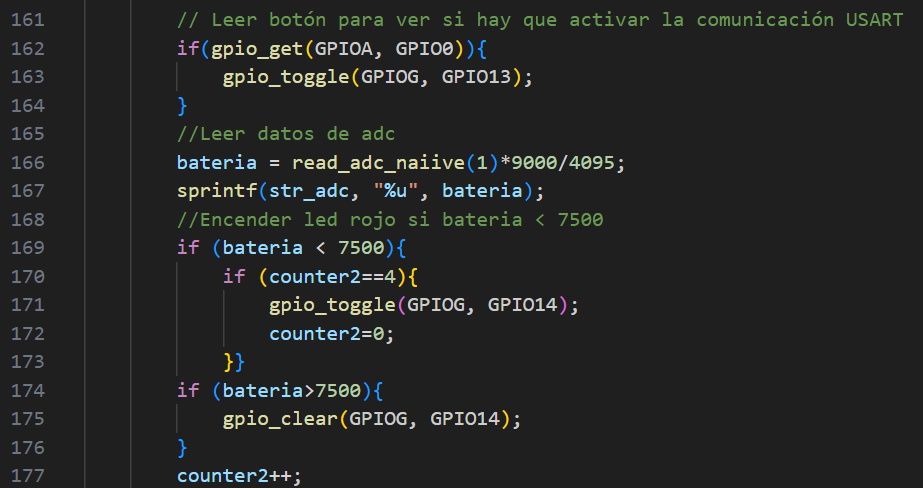
\includegraphics[scale=.6]{Imagenes/codig3.png}
    \caption{Código para controlar leds y comunicación.}
    \label{codig3}
\end{figure}

\subsection{Nivel de batería}
Para poder medir el nivel de la batería de 9V se puede utilizar un ADC de 12 bits incluido en la placa, pero primero es necesario condicionar la tensión de la batería a un rango seguro para la placa de 5V. Para esto se construyó un divisor de tensión utilizando las resistencias disponibles en la bodega, se opto por utilizar dos resistencias de 10k$\Omega$ y una de 2.2k$\Omega$. El siguiente diagrama muestra el circuito construido:
\begin{figure}[H]
    \centering
    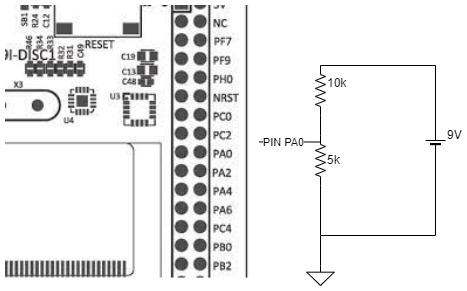
\includegraphics[scale=.7]{Imagenes/bateria (3).jpg}
    \caption{Esquemático del divisor de tensión. Diagrama de la placa tomado de \cite{discovery}}
    \label{fig:divisor}
\end{figure}

Como se muestra en la figura \ref{fig:divisor} la tensión de la batería pasaría a condicionarse a un nivel en donde la tensión máxima, es decir cuando la batería se encuentre a 9V, viene dado por:
\begin{equation}
    V_{out} = 9 \cdot \frac{5k}{10k+5k} = 3V
\end{equation}

De esta manera podemos conectar el pin PA0 al divisor de tensión de manera segura sin sobrepasar los limites de la placa. 

Ahora utilizando el ADC de 12 bits de la placa se configura para leer el nivel de tensión del pin PA1 y se obtiene un valor periódicamente que va de 0 a 4095. Este rango del ADC corresponde a un rango de tensión en el pin de 0 a 3.3V pero como calculamos anteriormente, el máximo valor de tensión que puede alcanzar a medirse en el pin es de 3V, gracias al circuito de acondicionamiento. Si realizamos un calculo rápido podemos ver que este valor corresponde a 3723 en el rango del ADC:
\begin{equation}
    3V \cdot \frac{4095}{5} = 3722.72
\end{equation}

El ADC en este caso nos daria mediciones en un rango 
de 0 a 3723, tomando esto en cuenta se puede mapear el valor a un rango de 0 a 9V nuevamente para obtener finalmente el nivel de tensión de la batería. Para mapear el valor a este nuevo rango simplemente se multiplica por 9 y se divide entre 3723 el valor obtenido del ADC.

En nuestro caso no fue posible encontrar un adaptador adecuado para conectar la batería y realizar el circuito, pero el código necesario para medir la tensión de la batería utilizando el divisor de tensión diseñado se puede encontrar en el repositorio del laboratorio. 

\subsection{Dashboard en ThingsBoard}
El primer paso para enviar los datos al dashboard de ThingsBoard es leer los datos enviados por la placa, para esto se establece conexión creando un objeto de tipo Serial() con el puerto serial que en este caso corresponde a ‘COM14’ con una tasa de 115200 baudios. 
Para enviar los datos al dashboard de ThingsBoard primero fue necesario agregar un dispositivo y generar un token necesario para realizar la conexión al host. Luego es necesario crear un objeto de tipo ‘mqtt.Client()’ y especificarle el host y el puerto para iniciar un loop infinito en donde se leen los datos del puerto serial y se ‘parsean’, es decir que se ordenan y se extraen los datos de los ejes, así como el nivel da la batería. Estos datos se utilizan para formar un diccionario el cual se envía como un objeto de tipo ‘json’ mediante la función ‘publish’.

A continuación se muestra el código utilizado: 
\begin{figure}[H]
    \centering
    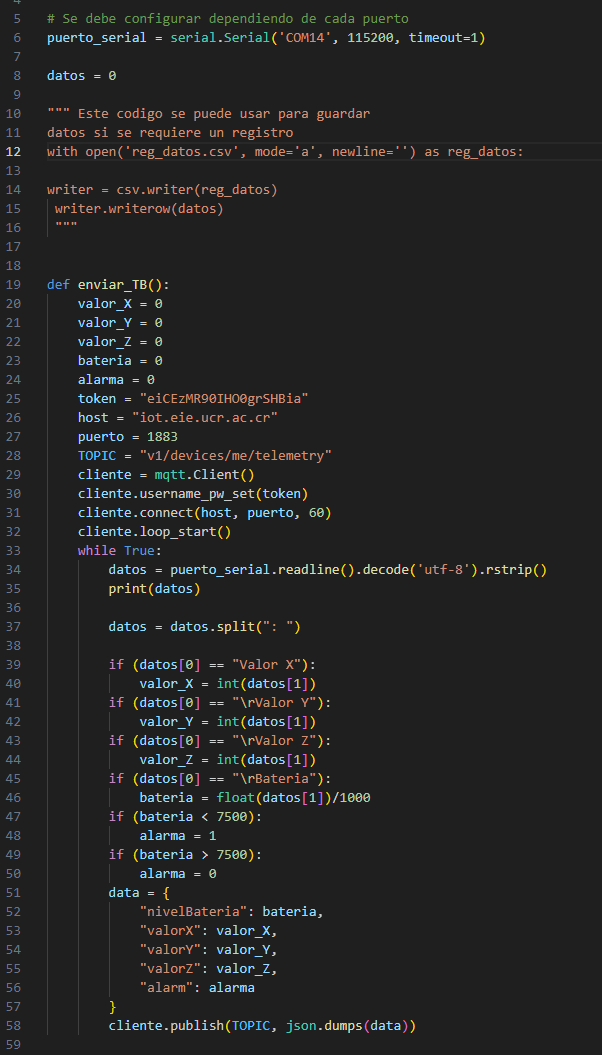
\includegraphics[scale=.7]{Imagenes/python.png}
    \caption{Script para leer y enviar datos a ThingsBoard}
    \label{fig:py}
\end{figure}


